\documentclass[a4paper,11pt,twoside]{book}
\usepackage{mythesis}
\usepackage{appendix}

%\usepackage[english]{babel}
%\usepackage[latin1]{inputenc}
%\usepackage{subfig}
%\usepackage{array}
%\usepackage{amsmath}
\usepackage{longtable}
\usepackage{color}
\usepackage{colortbl}
\usepackage{bibtopic}
%\usepackage{hyperref}

%\usepackage{url}


\makeindex
\setcounter{secnumdepth}{3}

\begin{document}

\title{title}
\author{Matteo Marini}

\universita{Politecnico di Milano}
\facolta{Ingegneria dell'Informazione}
\corsodilaurea{Ingegneria Informatica}

\relatore{Prof. William Fornaciari}
\correlatore{Ing. Patrick Bellasi}
\aacc{2009-2010}

\maketitle

\cleardoublepage

\newpage
\pagenumbering{roman}
\setcounter{tocdepth}{2}
\tableofcontents

\cleardoublepage 
\newpage
\pagenumbering{arabic}

\chapter{Introduction}
\label{cha:Introduction}

In the quest for the highest CPU performances, hardware developers have to deal with a difficult dilemma. On one hand, Moore's Law does not apply to 
computational power any more, that is, computational power is no longer doubling every 18 months as in the past. On the other hand, power consumption 
continues to increase more than linearly with the number of transistors included in a chip, and Moore's Law still holds for the number of transistors 
in a chip.
Several solutions have been adopted to solve this dilemma. Some of them try to reduce the power consumption by sacrificing computational power,
usually by means of frequency scaling, voltage throttling, or both. Other solutions try to increase the Instruction Level Parallelism (ILP) inside a 
processor, in order to get more computational power from the CPU without increasing power consumption. But nowadays the penalty of a cache miss 
(which may stall the pipeline) or of a miss-predicted branch (which may invalidate the pipeline) has become way too expensive.
Already in the early 2000's, it was clear that the most effective way to increase computational power and reduce power consumption was to parallelize
task execution. For this reason Simultaneous MultiThreading (SMT) was introduced. It is a technology that allowed to execute 
concurrently two threads on the same CPU. Nowadays it was introduced multicore
technolgy that consist of N superscalar processors put in the same chip. This tecnology allows a great parallelization of task execution.
With reference to memory organisation, multiprocessor systems are classified into two groups:

\begin{itemize}
	\item Centralised Shared Memory Architectures: in this architecture, there are multiple cores connected to a single shared memory. If all cores are
	      equal this architecture is called simmetric multiprocessor (SMP)
	\item Distributed Memory Architecture: in this architecture each processor has its own memory module and memory access time depends on the memory 
	      location relative to a processor. Non-uniform memory access (NUMA) processor are included in this category of architecture
\end{itemize}

Multicore architectures have been adopted by most chip manufacturers. Dual-core chips are commonplace, and numerous four and eight core options exist. 
In the coming years, per-chip core counts will continue to increase: Intel has claimed that it will release 80-core chips as early as 2013. 
The shift to multicore technologies is a watershed event, as it fundamentally changes the "standard" computing platform in many settings to be a 
multiprocessor.

Even many embedded systems are starting to adopt multicore architectures, because theese processors can provide a large increment of computational power,
with small increase in power consumption, that is a very important aspect for this type of systems.
But there is an obstacle to the use of these architectures in this sector and in particular in Real-Time systems.
In most multicore platforms, different cores share onchip caches. Imagine this situation: there are three Real-time tasks: A, B and C. 
A uses 512KB of memory, B uses 768KB and C uses 256KB. Our platform has a dual-core chip. Shared onchip cache is of 1MB.
There are two possible case of scheduling. In first case A and C (or B and C) are scheduled. There is enough space in cache to alloc their resources, 
and it is good. In the second case A is scheduled with B: cache trashing occurs. Performance of two tasks could get worse respect the previous case, because 
there isn't any guarantee that A or B may find data in shared cache and, furthermore, it is impossible to predict A or B duration, because if A is 
scheduled with B, it will have a certain duration. Instead, if A is scheduled with C, it will have another duration.
In other words: a task's duration depends from which other task is scheduled with it and, for this reason, using common Real-Time scheduling algorithms in 
multicore systems, well developed techinques for timing analysis of embedded software used in single processor systems are no loger useful, therefore 
new techinques are needed to estimate the worst-case execution time (WCET) of Real-Time tasks for this kind of platforms. 
It is clear that the scheduler plays an important role to improve performance and predictability of the applications. Nowadays, it is 
important to develop scheduling algorithms "cache-aware", that is a scheduler
that, to choose on which cpu to put a task, it consider  about how scheduled 
tasks use cache memory, in order to avoid cache trashing.
This thesis is the prosecution of the work carried out by Lucas De Marchi. He has tried to make the Linux Real-Time scheduler cache-aware
introducing the concept of taskaffinity. In this work, I have tried to improve the concept of taskaffinity and I 
have studied the behaviour of this mechanism on different multicore architectures.

\section{State of the art}
\label{sec:StateOfTheArt}

Although the problem to design "cache aware" scheduling algorithms is an old and well-known problem for over 20 years and multicore processors are 
largely used, nowadays operating systems don't implement this kind of algorithms and in literature there are only a few works that study this problem. 
The most of recent research works related to this argument consist of profiling activities with the aim to demonstrate and build a model that show how
an unfair cache sharing between concurrent threads may slow down them and cause sub-optimal throughput, cache trashing and, in some cases, thread 
starvation for threads that fail to occupy sufficient cache space to make good progress.
The first well-documented work related to this kind of scheduling algorithms, was developed at the Stanford University.
At the end of 80's, the Computer Systems Laboratory at Stanford University designed a prototype of a shared-memory multiprocessor called DASH. 
Its architecture was very similar to that used in modern SMP processors. DASH was able to incorporate up to 64 high-performance RISC microprocessors. 
In order to exploit full potentiality of this machine, they developed a suitable
runtime system to use with DASH, and they designed the COOL language. 
It was an extension of C++, that introduced some statements to facilitate expression of medium to large grain parallelism and to define which was the 
\textit{data reference patterns} of the program.
The COOL compiler was able to automatically extract fine-grain parallelism for architectures that, like DASH, supported such a level of concurrency,
and extract information about use of cache made by applications. Using these informations, the runtime system could ensure parallelism desired by 
programmer and try to reduce cache miss rate of each task, because this system "knew", for each task, which were the objects referenced by it, so 
it distributed tasks and objects in order to make them close.
In plain words, using additional informations provided by the programmer and exploiting the principle of data locality, the runtime system decided where to 
allocate objects and it assigned a task to a CPU that contained objects referenced by it in its cache. The COOL project shows how the smart use of cache 
is a problem that involves all aspect of software engineering, from the compiler to scheduler and memory management system.

Interesting research activities made in recent years exploit another strategy. They don't introduce new programming language or sophisticated runtime 
environment, but they implement a raw profiler that, at runtime, it infers how much cache space a task requires, in order to infer which 
tasks could cause cache trashing if they would be executed concurrently.
To make this job, the profiler executes a periodical tuning phase in which it analyzes miss rate of each task, in this way it is possible understand the 
amount of space used by a task. According to these informations, two or more
task are scheduled on different CPUs only if 
they don't cause cache trashing. These works are not effective as COOL project, but they present good results with SPEC2000 and 
LITMUS \footnote{It is a Linux-based testbed developed by them that supports multiprocessor real-time scheduling policies within Linux} benchmarks, 
furthermore this kind of works was experimented with good outcome also in embedded systems.


\section{Objectives of this thesis work}
\label{sec:ObjectiveOfThesis}


\section{Organization of the thesis}
\label{sec:OrganizationThesis}





\cleardoublepage
\chapter{Introduction to Cache Aware scheduling}
\label{cha:Rev_Presentation}

%TODO mettere citazioni per Kim, Calandrino, Fedorova Chandra molka usando \cite
In most multicore platforms, different cores share onchip caches, usually is L2 or L3 cache. Recent research works show how an unfair cache sharing
among concurrent tasks and cache trashing degrades performance. Modern operating systems (OS), attempt to schedule threads in a
fair and low-overhead manner.
Most simply, they balance the load across processor by migrating task to keep the run queues approximately equal. An OS assumes that,
in a given timeslice, resource sharing uniformly impacts the rates of progress of all the co-scheduled threads.
Unfortunately this assumption is often unmet because a thread's ability to compete for cache space is determined by its temporal reuse behavior,
which is often very different compared to that of other threads which are co-scheduled with it.

An interesting work developed by S. Kim et al. shows the impact of an unfair cache sharing on performance and how this phenomena is dependent by
co-scheduled threads. In Figure \ref{fig:gzip_miss} is represented one of results provided by that work.

\begin{figure}[htbp]
\centering
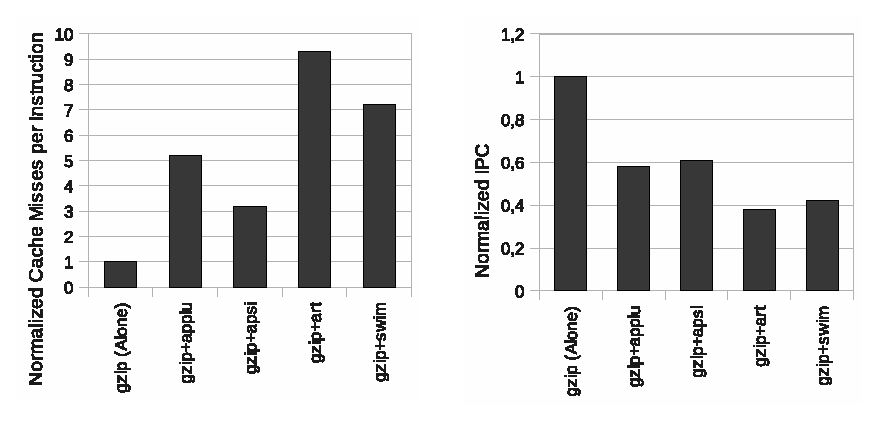
\includegraphics[width=\widefigure]{images/chandra_gzip}
\caption{\figurecaption{gzip miss rate}}
\label{fig:gzip_miss}
\end{figure}

The picture shows gzip's number of cache misses per instruction and instruction per cycle (IPC), when it runs alone compared to when it is
co-scheduled with different threads, such as applu, apsi, art, and swim. All the bars are normalized to the case where gzip is running alone.
It is interesting to note how gzip's number of cache misses per instruction increases significantly compared to when it runs alone. Infact, it increases 
by 3x when it runs with apsi and by 9.5x when it runs with art, 7.3x when it runs with swim.
Consequently, the IPC is affected differently. It is reduced by 35$\%$ when gzip runs with apsi, but reduced by 63$\%$ when gzip runs with art. 
Although not shown in the figure, art, apsi, applu, and swim's cache miss per instruction increases less than 15$\%$ when each of them runs with gzip. 

In terms of fairness, gzip's significant slow down can easily result in \textbf{priority inversion}. 
For example, if gzip has a higher priority than art, for gzip to achieve a higher progress rate, it has to be assigned more than three times the 
number of time slices compared to that assigned to art. Otherwise, to the end users, gzip may appear to be starved. In terms of throughput,
gzip's significant slow down reduces the overall throughput because the utilization of the processor where gzip runs on is also significantly reduced. 
Furthermore, it is possible that the co-scheduled threads's working sets severely overflow the cache and create a \textit{trashing} condition.

In briefly, there are at least three problems that may happen and render the OS schedule ineffective.
The first problem is \textit{thread starvation}, which happens when one thread fails in competing for sufficient cache space necessary to make 
satisfactory forward progress. The second problem is \textit{priority inversion}, where a higher priority thread achieves a slower forward
progress than a lower priority thread, despite the attempt by the OS to provide more timeslices to the higher priority thread.
This happens when the higher priority thread loses to the lower priority thread (or other threads) in competing for cache space. 
To make things worse, the operating system is not aware of this problem, and hence cannot correct this situation (by assigning more timeslices to the 
higher priority thread). The third problem is that the forward progress rate of a thread is \textit{highly dependent} on the thread mix in a co-schedule. 
This makes the forward progress rate difficult to characterize or predict, making the system behavior unpredictable. Unfortunately, despite these problems, 
cache implementations today are thread-blind, producing unfair cache sharing in many cases.

As I said in the first chapter, in theese years were developed some ideas about how to make a scheduler cache-aware.
This chapter aims to show the general structure and strategies used to model cache behaviour followed by theese algortihms, that are the most interesting 
part of theese type of heuristics.

%%%%%%%%%%%%%%%%%%%%%%%%%%%%%%%%%%%%%%%%%%%%%%%%%%%%%%%%%%%%%%%%%%%%%%%%%%%%%
\section{Structure of Cache aware Scheduling}

Before to explain how theese algortihms work, it is necessary to pay attention to which are assumptions made by theese heuristics about type of application 
and platform considered.

Assume a multicore platform consisting of $M$ cores that sharing an on-chip Last Level cache divided in $A$ partitions, and a task set $\tau$,
in which each task $T$ releases a job $J_i$ every period $p(T)$, and every released job is characterized by a worst-case execution time (WCET) denoted
by $e(T)$. This means that each job released by task $T$ has a maximum duration of $e(T)$. For each job is defined the number $A(J_k)$ that represents 
number of cache partitions, and then the total cache space size, used by it. For simiplicity we assume that each job generated by a task $T$ use the same
number of partition, therefore it is possbile to express $A(J_k)$ as $A(T)$.
The quantity $e(T)/p(T)$ is called the utilization of $T$, denoted $u(T)$. The deadline $d(J_k)$ of a job $J_k$ coincides with the release time of job 
$J_{k+1}$. If job $J_k$ completes its execution after time $d(J_k)$, then it is tardy. For some scheduling algorithms, tardiness may be bounded by some 
amount $B$, meaning that any job $J_k$ will complete execution no later than time $d(J_k)+B$. 

In this model we don't take care about core-local cache (usually L1) or other shared resources like interconnects are not modelled.
We assume the existence of a cache partitioning mechanism, allowing to divide the cache space into non-overlapping partitions. 
In this way, we know how many partitions, and then how many space, a task requires to execute its work. The model is very adapt to represent Real Time tasks.

\newpage

%-----------------------------------------------------------------------------
\subsection{The policy of the scheduler}

This kind of algorithms are a variant of classic scheduling algorithms, beacause they mantain the same characteristics, such as priority inheritance etc.,
and in addition they take care about which is memory region used by scheduled tasks. All heuristics analyzed follow theese rules: a job $J_k$ is 
scheduled for execution if:

\begin{enumerate}
	\item $J_k$ is the job of highest priority among all waiting jobs,
	\item There is at least one core idle
	\item There are enough cache partitions, i.e. at least $A(J_k)$ , are available.
\end{enumerate}

\begin{table}[htbp]
\begin{center}
\begin{tabular}{l|c|c|c}
	\hline
	& $p(T)$ & $C(T)$ & $A(T)$ \\ \hline
	$T_1$ & 3 & 2 & 1 \\ \hline
	$T_2$ & 4 & 3 & 2 \\ \hline
	$T_3$ & 5 & 3 & 2 \\ \hline
	$T_4$ & 8 & 3 & 1 \\ 
	\hline
\end{tabular}
\caption{An example task set}
\label{tab:cache_task_set}
\end{center}
\end{table}

\begin{figure}[htbp]
\centering
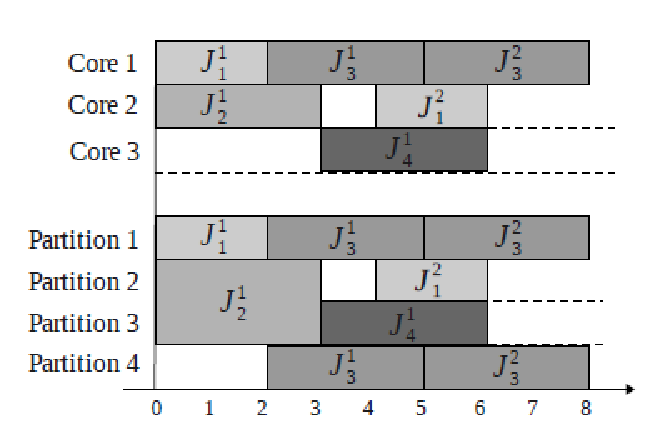
\includegraphics[width=\widefigure]{images/schedule.eps}
\caption{\figurecaption{Example of scheduling performed by cache aware policy}}
\label{fig:sched_example}
\end{figure}


Figure \ref{fig:sched_example} shows how the task set in Table \ref{tab:cache_task_set} is scheduled by our cache aware policy. The index of each task 
indentify the task and indicate the priority of the latter. Higher priority is 1 and lower priority is 4. In the picture jobs are represented in this way: 
$J_{\alpha}^\beta$, where $\alpha$ represents which task has released the job, and then also its priority, and $\beta$ is an index that identify the job.
At time 0 all jobs are released. At this time, the job $J_{4}^1$ can not be executed because it has lower priority than $J_{3}^1$ and the latter can not be
scheduled since there is not enough idle cache partitions available.

Analyzed algorithms implement this policy using different data structures and different strategies such as job promoting, variable time-slice etc., but 
the real differences between analyzed heuristics, are metrics and methods used to estimate which are the cache partitions requested by each task or
thread to schedule.

%-----------------------------------------------------------------------------
\section{Methods to infer cache space used}

As seen in the previous section, an hypotesis made in our application model is to have a mechanism, that we will call co-scheduler, that computes how many 
space each task requires. According to defined policy, the scheduler use theese informations and schedule tasks in order to avoid cache trashing.
In the development of this kind of scheduler, the real challange is to build an efficient co-scheduler that, at runtime, provides necessary informations.
In theese years, a lot of model to study cache behaviour in multicore systems were developed. In the majority, they are used as a profiling tool for
applications and not to implement cache aware scheduling heuristics %TODO ref al dynamic cache partition.
But some interesting works developed by Calandrino and Fedorova show how it is possible to build empirical and effective cache behaviour model
according to "low-cost" information suitable to implement a co-schedule systems. This works can be applied for both Real-time and general-purpose systems.

%-----------------------------------------------------------------------------
\subsection{Methods applied for Real-time systems}

Works developed by Calandrino et al. is focused on multimedia soft real-time application. In this work, tasks are multithreaded tasks applications (MTTs),
this hypotesis don't damage generality of the application model presented in the previous section.
Co-scheduler proposed is a profiler that provides a per-job working set sizes (WSS) estimate for each MTT. The per-job WSS of an MTT indicates the amount 
of memory referenced by all tasks of that MTT while executing one "job" of the MTT, where the ith job of an MTT consists of the ith jobs of all tasks 
in the MTT. It profiles MTTs rather than tasks since MTTs share a common working set. 
The profiling occurs during job execution, eliminating the need for and offline profiling tool. WSS may be seen as an oversimplification of 
cache behavior; but it to work well for small intervals (e.g., the execution time of a job). Further, it is usually the easiest metric to 
approximate efficiently given current hardware.

The profiler as stated requires some additional assumptions:

\begin{enumerate}
\item Each job of the same task is assumed to perform roughly the same operations on different (but similarly-sized) sets of data.
      This has two implications: (a) the ith job of task T and the j th job of task U , where T and U belong to the same MTT, do not share
      significant data unless i = j (even if T = U ); and (b) the per-job WSS of an MTT remains approximately the same over all jobs.

\item Profiled jobs are not preempted and do not cause shared cache thrashing.

\end{enumerate}

The first assumption is natural for certain types of (multimedia) applications. To ensure latter assumption, it is necessary discard measurements obtained
for jobs that are preempted, or for which cache thrashing occurred at some time during their execution. 
Thrashing is assumed to have occurred if for some quantum in which a job is scheduled, the sum of the WSSs of all MTTs with jobs scheduled in that quantum 
exceeds the shared cache size. For MTTs, measurements for the ith job of all thread in the MTT must be discarded if the $ith$ job of any thread in the 
MTT was preempted or caused thrashing.
Furthermore, the second assumption also implies that it is not interesting to profile MTTs with per-job WSSs greater than the size of the
shared cache, which would thrash the shared cache even if scheduled in isolation.

The above assumptions allow us to compute over all (non-discarded) jobs an average per-job MTT WSS, which it can be used as per-job WSS estimate for
an MTT. This can be computed by dividing the total shared cache misses observed over all profiled jobs by the total number of profiled jobs for an MTT, 
and multiplying the result by the cache line size.

But, how can it is possible to measure shared cache misses? Thanks to performance counters.
A performance counter for each core is programmed to track lower-level shared cache. Since jobs execute sequentially, it is possible to measure the number
of cache misses incurred for a job by resetting the counter to zero at the start of execution, and recording the total misses observed by the counter
upon completion. The observed misses can then be used to calculate a per-job WSS estimate. Since accessing program counters and recording data
are low-overhead operations, and computed WSS estimates are cached to minimize computation, the overhead of the profiler is relatively low.
It is clear that at the begin of a MTT, there isn't any measure about its miss rate. For this reason, profiler need of a initial tuning phase, in which an 
estimate of all MTT's WSS is done. This phase converge pretty fast to a reasonable result. For details see %TODO Calandrino 

%-----------------------------------------------------------------------------
\subsection{Methods applied for general purpose systems}

Co-scheduler developed by Fedorova et al. consider generic multithreaded tasks that can be preempted or not, it is not focused on soft Real-time 
applications. 

Their approach is based on an empirically observation that if the co-runners have similar cache miss rates they share the cache
roughly equally. So if co-runners A and B experience similar miss rates, they share the cache equally and they each experience their
\textbf{fair miss rate}. In this case, A and B are cache-friendly co-runners.

The fair miss rate is the number of misses per cycle (MPC) that would be generated by a thread if the cache were shared equally. This is metric used
to determine the best grouping between task.

Procedure to estimate the fair cache miss rate for each thread is very simple.
For each thread to profile, call it Thread A, execute it with several different co-runners and derive the relationship between its miss rate and 
miss rate of its corunner. This relationship is used to estimate the miss rate that Thread A would experience with a "hypothetical" 
cache-friendly co-runner; this miss rate is Thread A's fair miss rate. 

\newpage

\begin{figure}[htbp]
\centering
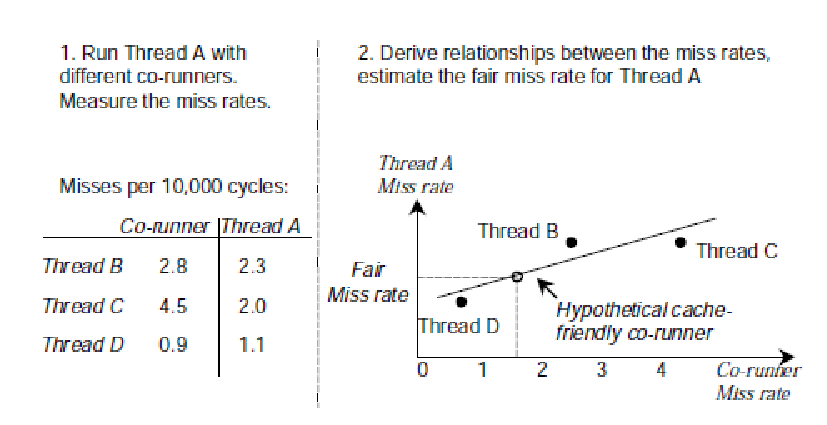
\includegraphics[width=\widefigure]{images/fedorova.eps}
\caption{\figurecaption{fedorova temp}}
\label{fig:fed}
\end{figure}

Figure \ref{fig:fed} illustrates this idea. Step 1 shows the miss rates measured as Thread A
runs with different co-runners. Step 2 shows that exists a linear relationship between the miss rate of Thread A and its co-runners.
We use the corresponding linear equation to compute Thread A's miss rate when running with a hypothetical cache-friendly co-runner - its fair miss 
rate.

This strategy is based on two important assumptions 
\begin {enumerate}
	\item Cache-friendly co-runners have similar cache miss rates.
	\item The relationship between co-runners' miss rates is linear.
\end{enumerate}

The former is true, because if each thread's shared cache accesses are uniformly distributed in the cache, it is possible to model cache 
replacement as a simple case of the balls in bins problem, that is: assume two co-runners, whose cache requests correspond to black and white balls 
respectively. We toss black and white balls into a bin. Each time a ball enters the bin, a ball is evicted from the bin. 
If we throw the black and white balls at the same rate, then the number of black balls in the bin after many tosses will form a
multinomial distribution centered around one-half. This result generalizes to any number of different colored balls being tossed at
the same rate. Thus, two threads with the same shared cache miss rate (balls being tossed at the same rate) will share the cache equally.
It is important to remark that this assumption is true only if cache request are uniformly distributed. Fedorova et al. have measured cache requested
made by SPEC2000 benchmarks, and they have found that for most benchmarks, the distribution was close to uniform, so it is correct using the balls in bins
problem to represent cache replacement

The latter assumption is demonstrated by this experiment.
They chose nine benchmarks from the SPEC CPU2000 suite with different cache access patterns and ran them in pairs on their simulated dual-core processor.
They ran each benchmark in several pairs. They analyzed the relationship between the miss rate of each benchmark and the miss rates of its co-runners and 
found that a linear equation approximated these relationships better than other simple functions.

The expression for the relationship between the co-runners' miss rates for a processor with $n+1$ cores is:
\begin{equation}
	MissRate(T) = a*\sum_{i=1} MissRate(C_{i}) + b
\label{eq:miss_rate}
\end{equation}

where,
\begin{enumerate}
	\item $T$ is a thread for which they compute the fair miss rate
	\item $C_i$ is the $i-th$ co-runner
	\item $n$ is the number of corunners
	\item $a$ and $b$ are the linear equation coefficients
\end{enumerate}

Thread $T$ experiences its fair cache miss rate $FairMissRate(T)$ when all concurrent threads experience the same miss rate, therefore:

\begin{equation}
	FairMissRate(T) = MissRate(T) = MissRate(C_i)
\end{equation}

for all $i$. Equation \ref{eq:miss_rate} can be expressed as:

\begin{equation}
	FairMissRate(T ) = a*n*FairMissRate(T) + b 
\end{equation}

where the expression for $FairMissRate(T)$ is:

\begin{equation}
	FairMissRate(T) = \frac {b}{1-a*n}
\end{equation}

The co-scheduler implemented dynamically derives coefficients for Equation 1 for each cache-fair thread at runtime and then estimates its fair cache 
miss rate. Also in this case, cache misses are retrived using performance counters, expressly programmed. Further, also this method requires a periodical 
tuning phase used to account thread's cache access pattern.

Showed approches are similar, but present some differences.
First of all, they are focused on two different type of tasks: first approach considers Real-Time tasks, the latter considers fair tasks.
Test environments are different. Calandrino et al work is Linux based, they used LITMUS benchmarks suite and they tested their work on Intel i7.
Fedorova et al. work is Solaris based, they used SPEC2000 benchmarks and they tested on a simulator of UltraSPARC T1
Both strategies try to understand how scheduled thread use shared cache, but they do this job in different way: the first method is focused only
to prevent cache trashing, the latter is more complex: it tries to prevent cache trashing too, furthermore it tries to understand how two co-scheduled
threads use shared cache.

Calandrino and Fedorova show in their papers how their works reduce shared cache miss and how this fact improve execution time (and predictability)
of benchmarks tested.

\section{Survey on cache architecture}
\label{sec:s1}

Over the years, cache architectures have always played an important role in system performance. Hundreds of research papers show how performance
can be improved using multi-level caches on a single-processor machine. Multicore systems introduce new challanges for cache designer, because cache memory 
is a shared resource, therefore issues related to how a core access to cached data and how the coherence regarding the access from different processors 
to the same cached data is guaranted are unavoidable. Furthermore, caches play an important role in managment of comunication betwen different core.
This section aims to show which are most important factors introduced in cache architecture to take in consideration during the development of cache aware
alogrithms from scratch. Theese cache characteristics are common in both general purpose and embedded systems.

%-----------------------------------------------------------------------------
\subsection{Cache coherent protocols}

Usually in multicore architecture, there is a private L1 cache for each core, and there is a L2 or L3 cache shared among all cores (SMP), or among cores 
that belong to the same node (NUMA). Shared cache is one of the most critical resources in multicores.

\begin{figure}[htbp]
\centering
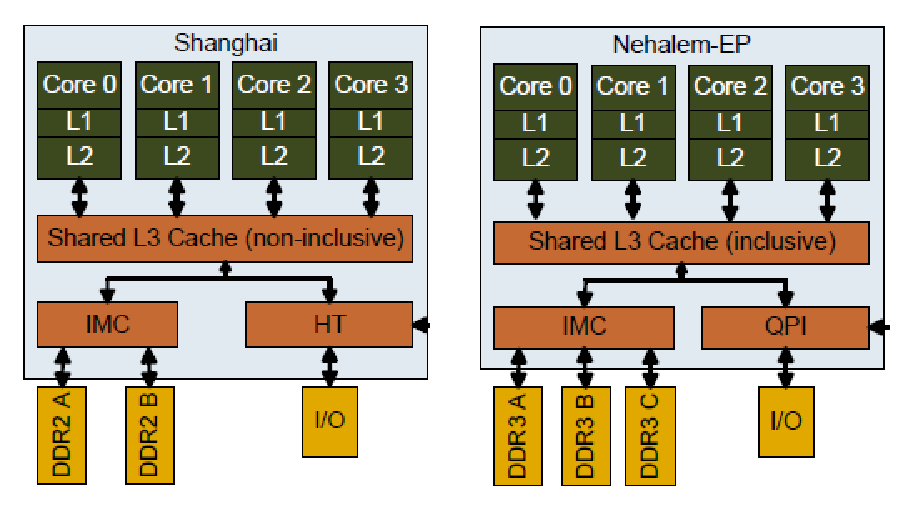
\includegraphics[width=\widefigure]{images/neh_amd.eps}
\caption{\figurecaption{Intel nehalem and AMD Shanghai}}
\label{fig:neh_amd}
\end{figure}

As for all types of shared resources, also for shared cache it's necessary to ensure integrity of the shared data.
Before to analyze mechanisms used to ensure data integrity, it is necessary pay attention to the difference between two terms: consistence and coherence.
When two or more CPUs operate on a shared variable and one of these CPUs modify the variable, it is necessary that the information regarding
this change of value be communicated to the other CPUs. Consistence refers to 'when' this change in memory data is available to other CPU cores.
Coherence refers to 'how' the change is communicated between the processors. Therefore, to ensure correctness of cache operations, it is necessary define
when a modified value must be made visible to another processor's read instruction, this is the consistency model, and define the rules used to comunicate 
memory update between different cores, this is coherence protocol. In briefly a cache coherence protocol is the mean used to maintains consistency between
all the cache in the system.
Existing coherence protocols are classified based on the mechanism by which they ensure cache coherence: 

\begin{itemize}

\item Snooping based protocols: Each cache monitors address lines of shared bus for every memory transaction made by remote processors. Appropriate action
is undertaken when data locally cached is modified by this transaction, for example: a write by a remote processor into a data address locally cached 
results in an invalidation of the local cache copy .

\item Snarfing based protocols: A cache controller watches both address and data in an attempt to update its own copy of a memory location when a second 
master modifies a location in main memory. When a write operation is observed to a location that a cache has a copy of, the cache controller updates its 
own copy of the snarfed memory location with the new data.

\item Directory-based protocols: Shared data are placed in a common directory that maintains the coherence between caches processor caches. 
This directory acts as a look-up table for every processor to verify coherence and consistency of data that is currently being read or updated.

\end{itemize}


The first two mechanisms are typical of the SMP architecture, while the last is used in large point-to-point inter-processor communication network 
architectures. Snooping protocols became popular and widely accepted with multiprocessors systems since it required minimal change to the pre-existing 
physical shared bus interface to the memory. The inherent broadcasting property of the snoop protocols makes it simple to implement but places an upper 
limit on scalability.
Over the years, several snooping based cache coherence protocols were developed. The most common is MESI protocol.
With this protocol, every cache line is marked with one of the following states:

\begin{itemize}

\item Modified
The cache line is present only in one of the local caches, and it has been modified from the value in main memory. Write on a modified cache line are 
allowed, reads are a bit complicated. The local cache that owns a modified cache line must intercept (snoop) all attempted reads (from all of the other 
caches in the system) at main memory location that correspond to modified cache line, forcing them to back off, then writing data to main memory and change
state of cache line to shared state.
 
\item Exclusive
The cache line is present only in the current cache, and it matches main memory. It is possible read/write lines in this state. A cache that own
line in exclusive state must snoop all read transaction from all other cache and if it intercepts some read that regard owned cache line, it changes
state of that line from exclusive to shared.

\item Shared
Indicates that this cache line may be stored in other caches and it matches the main memory. It is possible read cache line in this state. Writes to a shared
cache line are allowed but before to perform the operation, it is necessary invalidate all other copies in other caches.
A cache that holds a line in the Shared state must listen for invalidation from other caches, and discard the line (by moving it into Invalid state) on a 
match.

\item Invalid
Indicates that this cache line is invalid, read/write operation on invalid cache line are denied

\end{itemize}

Cache coherence protocols play an important role to improve efficiency of the read/write in cache. There are a lot of variant of MESI protocol, the most 
recent variants are MESIF and MOESI.

The former protocol adds Forward state. It is only relevant for the L3 cache. This state indicates that only one cache should act as a designated responder 
for any requests for the given line. With the standard MESI protocol, a request for cache line will receive a response from each cache that contains that 
line in the shared state. Instead, with MESIF protocol a request will be responded to only by the cache holding the line in the Forward state.
A cache line shared among multiple processors will be in forward state in only one L3 cache. This protocol is used in new Intel microarchitecture Nehalem 
and it is designed for ccNUMA. The aim of this new state is to reduce communications between cache.

The latter protocol add Owned state. A cache line in this state holds the most recent, correct copy of the data. Only one processor can hold the data 
in the Owned state, all other processors that contains a copy of that data must hold the them in the shared state. A copy of data in main memory can be 
incorrect. A cache line in owned state may be changed to the Modified state after invalidating all shared copies, or changed to the Shared state by 
writing the modifications back to main memory, furthermore cache lines must respond to a snoop request with data. 
It is clear that the aim of this protocol is to avoid the need to write a dirty cache line back to main memory when another processor tries to read it. 
With the Owned state, processor can supply the modified data directly to the other processor. This is beneficial when the communication latency and 
bandwidth between two CPUs is significantly better than to main memory. An example of MOESI implementation is present in AMD Shanghai microprocessor.

%-----------------------------------------------------------------------------
\subsection{Inclusive and exclusive cache}

Another important architecture detail that affect performance is if a cache is inclusive or exclusive.
An inclusive cache means that all data available in higher level cache are contained also in the last level cache, namely in shared cache.
An exclusive cache means that data is present only in one cache.

It is clear that theese two architectural policy are focused on two different aspects. The first policy greatly reduces snoop traffic because if a core 
doesn't find requested data in any of its cache level, it knows the data it is also not present in any other core's cache. The second policy, instead, 
allows to store more data than an inclusice cache, because for each data only one copy is stored.

An example of inclusive L3 shared cache is implemented in Intel Nehalem microarchitecture. In this implementation to insure coherency across 
all caches, the L3 cache line has additional flags that keep track of which core the data came from and a core valid bit that indicate that cache line 
is present in some core's cache. If the data is modified in L3 cache, then the L3 cache "knows" if the data came from a different core than last time 
and that the data in the first core needs its L1/L2 values updated with the new data. This greatly reduces the amount of traditional "snooping"
coherency traffic between cores. Moreover the core valid bit doesn't ensure that a L3 cache line is placed also in an higher level cache, because unmodified
cache lines may be evicted from a core's cache without notification of the L3 cache.

An implementation of exclusive cache can be found in AMD's Shanghai processors. Theese cpus present an interesting implementation of this type of cache
architecture, because L1 and L2 are exclusive cache, but last level shared cache (L3) is a not-inclusive cache.
Not-inclusive architecture is a variant of exclusive architecture, becasue if a cache line is transferred from the L3 cache into the L1 of any core, the 
line can be removed from the L3. According to AMD this happens if it is "likely" that the line is only used by one core, otherwise a copy can be kept in 
the L3.
About how the cpu can "understand" if a line will be used only by one core, AMD has not revealed details.
Nowadays, an inclusive cache is preferred over an exclusive cache, because it simplifies the problem of cache coherence. 

%-----------------------------------------------------------------------------
\subsection{Cache Hardware prefetcher}

It is necessary to spend a few words about prefetching. Prefetcher is an hardware component that tries to predict which memory addresses are
going to be used by the program, in order to load needed data in cache memory just in time.
Typical technical workloads often access memory in regular and sequential patterns, therefore, with a smart prediction mechanism, a prefetcher can select 
and load right data and, in this way, reduce memory latency. The key point to build a good prefetcher is to design prediction mechanism.
In literature there are many ideas to solve this problem. An example of concrete solution is the Intel Smart Memory access. This system was introduced
with Intel Core microarchitecture. In this system there are two prefetchers to the Level 1 data cache and the traditional prefetcher to the Level 1 
instruction cache. In addition there are two prefetchers associated with the Level 2 cache and shared between the cores. In total, there are eight
prefetchers per dual-core processor. 
In order to improve the accuracy of the prediction, the prefetcher system tags the history of each load using the Instruction Pointer (IP) of the load. 
For each load, the prefetcher builds a history and keeps it in a suitable history array. Based on load history, the prefetcher tries to predict the 
address of next load accordingly to a constant stride calculation (a fixed distance or "stride" between subsequent accesses to the same memory area). 
At this point, the prefetcher generates a prefetch request with the predicted address and brings the resulting data to the Level 1 data cache.
In literature, this kind of prefetchers are called \textit{strided} prefetcher.
Other architectures, such as Power ISA\_2.06, that use a strided prefetcher, introduces cache instructions to hint prefetch system for data prefetching.
With this instructions an application can specify direction, depth, no of units and so on. In this way, the programmer has a low level control on 
data prefetched.

Another category of prefetcher are \textit{non-strided} data prefetcher. They are very useful for accessing complex and irregular data structures as 
linked list, B-Trees etc. There are different techniques to implement theese prefetcher, one of theese is "pattern history based prefetcher". 
In this approach, the prefetcher tracks the addresses of misses and tries to identify specific patterns of misses that occur together (temporally). 
Once a pattern of misses has been detected, the prefetcher will find the first miss in the pattern. When this first miss occurs again, the prefetcher 
will immediately prefetch the rest of the pattern. For traversing a complex data structure like a linked list, this would be a fairly effective approach.
Recently AMD has announced that it will employs a non-strided prefetcher in its brand new Bulldozer microarchitecture, but it has not revealed details on 
implementations.




\cleardoublepage
\chapter{Improve taskaffinity}
\label{cha:Improve taskaffinity}

TODO potevamo dire alla select di prendere il lock ma questo modificava troppo la logica del kernel, tenere un approccio self-contained
TODO dove si dice che il throughput si disfa dire che la predictability aumenta per\'o le migration dan fastidio
TODO richiamare la definizione di taskaffinity e dire cosa ricevono in input le syscalls
TODO occhio che la select non ha nessun lock
TODO ricordarsi che ci sono la push\_rt\_task e la pull-rt-task

In this chapter we present which are optimization performend and why. we see ... TODO 

%%%%%%%%%%%%%%%%%%%%%%%%%%%%%%%%%%%%%%%%%%%%%%%%%%%%%%%%%%%%%%%%%%%%%%%%%%%%%
\section{Scheduler architecture on 2.6.34}

Now I will briefly introduce which are the part of scheduling procedure interested by taskaffinity logic and which are the most important changes carried 
out from 2.6.31 kernel version to 2.6.34.

%-----------------------------------------------------------------------------
\subsection{Task wake up management}

The scheduling procedure for a task starts when it wakes up. A task can wake up
for different reasons, i.e. a semaphore becomes unlocked, task's creation
(in that case it has the first wake up), etc.. In all those cases different
kernel functions are called, but at the end they call 
\texttt{try\_to\_wake\_up} function. The API of \texttt{try\_to\_wake\_up} is:

\lstset{basicstyle=\footnotesize, language=c, captionpos=b, frame=single, label=lis:API\_ttwu}
\lstinputlisting{API_ttwu.c}

Where $p$ is the to be waken task, other input parameters are not important now.
This function follows these steps:

\begin{enumerate}
\item Disables kernel preemption, locks the runqueue where $p$ was last executed and check 
if $p$ is not already waken and if it is not already on a runqueue. In the first case the 
function releases lock and exit, in the second case the function check if a
\textit{push} is necessary, further details about these if statements will be
describe soon. If two checks fail, $p$'s state is changed, the lock on runqueue
is released and \texttt{select\_task\_rq}, a wrapper for a class-specific 
\texttt{select\_task\_rq\_rt}, is called. The function \texttt{task\_waking}
at line TODO line is class-specific and regards only Fair tasks.

\lstset{basicstyle=\footnotesize, language=c, captionpos=b, frame=single,label=lis:steps}
\lstinputlisting{ttwu_steps.c}

\item \texttt{select\_task\_rq\_rt} choose on which cpu $p$ will be executed. It
calls \texttt{find\_lowest\_rq} that returns the best cpu where to put $p$. What
is the best cpu for $p$ will be clear soon. When \texttt{select\_task\_rq\_rt} 
returns, check if selected cpu is online, in that case returns, otherwise calls
\texttt{select\_fallback} that returns an any online cpu that "respects" $p$'s 
cpu affinity.

\lstset{basicstyle=\footnotesize, language=c, captionpos=b, frame=single,label=lis:steps}
\lstinputlisting{select_task.c}

\item acquires the lock on selected runqueue, updates some $p$'s statistics, enqueues 
$p$ on selected runqueue, update $p$'s state in TASK\_RUNNING and call
\texttt{check\_preempt\_rq}

\lstset{basicstyle=\footnotesize, language=c, captionpos=b, frame=single,label=lis:steps}
\lstinputlisting{ttwu_check.c}

\item checks if $p$ has priority greater than priority of the task currently
executed on selected runqueue, in that case it calls \texttt{need\_resched}
function in order to perform the context-switch on selected runqueue at the
end of \texttt{try\_to\_wake\_up}.

\lstset{basicstyle=\footnotesize, language=c, captionpos=b, frame=single,label=lis:steps}
\lstinputlisting{check_prio.c}

\item call class-specific function \texttt{task_woken} to check if $p$ must be
pushed from the selected runqueue.

\lstset{basicstyle=\footnotesize, language=c, captionpos=b, frame=single,label=lis:steps}
\lstinputlisting{final_ttwu.c}

\end{enumerate}

The most important differences from version 2.6.31 related to Real-time tasks regard principally \texttt{try\_to\_wake\_up}. 

TODO figura comparativa codici

It is possible to have multiple istances of \texttt{try\_to\_wake\_up} for the same task executed simultaneously. In the 2.6.31 kernel version, this problem
is resolved by holding runqueue lock. In the 2.6.34 kernel version, to deal with this issue a new task's state named TASK\_WAKING was introduced. This state
is used to indicate someone is already waking the task, in this way other istances of \texttt{try\_to\_wake\_up} fails when executes the if statement at 
line TODO ref, because input parameter $state$ is in the most cases equal to TASK\_ALL and then, according to fig TODO stati,
\texttt{TASK\_WAKING & TASK\_ALL} return 0 and \texttt{try\_to\_wake\_up} exits. With this solution it is possible reduce time in which lock on runqueue is 
held. 


%-----------------------------------------------------------------------------
\subsection{Migration policy}

Another important part of scheduling procedure is the migration policy. Migration of Real-time tasks is made in two way: 

\begin{description}
\item[Push tasks:] The push operation is implemented by \texttt{push\_rt\_task()}. The function receives in input a runqueue and looks at the 
highest-priority non-running runnable real-time task on the input runqueue and considers all the runqueues to find a CPU where it can run. It searches for 
a runqueue that is of lower priority, that is, one where the currently running task can be preempted by the task that is being pushed. 

The research and the choice of the best cpu for the task to push is executed by \texttt{find\_lowest\_rq} the same function used in 
\texttt{select\_task\_rq\_rt}. This function builds a mask of cpus that have the lowest-priority runqueues and returns the cpu on which the task to push is 
last executed, as it is likely to be cache-hot in that location. If this is not possible, the \texttt{sched\_domain} map is considered to find a CPU that 
is logically closest to last cpu that has executed the task to push. If this too fails, a cpu is selected at random from the mask.

The push operation is performed until a real-time task fails to be migrated or there are no more tasks to be pushed. Because the algorithm always selects 
the highest non-running task for pushing, the assumption is that, if it cannot migrate it, then most likely the lower real-time tasks cannot be migrated 
either and the search is aborted. No lock is taken when scanning for the lowest-priority runqueue. When the target runqueue is found, only the lock of that 
runqueue is taken, after which a check is made to verify whether it is still a candidate to which to push the task (as the target runqueue might have been 
modified by a parallel scheduling operation on another CPU). If not, the search is repeated for a maximum of three tries, after which it is aborted. 

In order to decide which tasks must be pushed, a linked list named \textit{pushable\_list} is added to each runqueue. \texttt{push\_rt\_task()} selects task
to push from this list. A task is inserted in this list when it is enqueued on a runqueue see fig TODO snip enqueue. 

The current task of any runqueue can't never be in a pushable list, in fact, during a context switch the next task to be executed is removed from the 
runqueue's pushable list.

\item[pull task:] The pull operation is implemented by \texttt{pull\_rt\_task()}. The algorithm looks at all the overloaded runqueues in the system 
and checks whether they have a Real-time task that can run on the target runqueue (that is, checks if the target cpu "respects" the cpuaffinity of the 
task to pull) and if that Real-time task is of a priority higher than the task the target runqueue is about to schedule. If so, the task is queued on 
the target runqueue. This search aborts only after scanning all the overloaded runqueues in the system. 

\end{description}

In the 2.6.34 kernel version, the migration logic and all data structures involved are not changed from 2.6.31 version.

%%%%%%%%%%%%%%%%%%%%%%%%%%%%%%%%%%%%%%%%%%%%%%%%%%%%%%%%%%%%%%%%%%%%%%%%%%%%%
\section{Test computers}

In this work, all the test machines are quad-core 
systems and whenever. They have different cache configurations
as detailed below and illustrated in Fig.. Since they have different
power management solutions to scale the frequency, which could

TODO descrivere brevemente come sono fatte le macchine e dire che il numasauro usa lo shield ecc.

%%%%%%%%%%%%%%%%%%%%%%%%%%%%%%%%%%%%%%%%%%%%%%%%%%%%%%%%%%%%%%%%%%%%%%%%%%%%%
\section{Taskaffinity behaviour}

%-----------------------------------------------------------------------------
\subsection{Buffer sizes}

TODO far notare differenza latenze scheduling a 4KB ec.. calcolo incidenze
TODO magari qualcosa sui tempi 

%-----------------------------------------------------------------------------
\subsection{Migration issues}
TODO dire che c'\'e il ping pong e dei problemi che la migration comporta per il warm up della cache, dire che i 2 banchi di cache sullo Xeon sono
TODO un casino

%-----------------------------------------------------------------------------
\subsection{Cache misses}

TODO stesse considerazioni per dar ragione alle considerazioni fatte per le migration
TODO scrivere evento che si va a registrare, magari dicendo che perf pensa a fare tutto quel che serve 

TODO i cache miss e i tempi medi di esecuzione

TODO dire come a 32KB la cache non conti niente

%%%%%%%%%%%%%%%%%%%%%%%%%%%%%%%%%%%%%%%%%%%%%%%%%%%%%%%%%%%%%%%%%%%%%%%%%%%%%
\section{Patch structure}

TODO serve introdurre la definizione di taskaff di lcs e richiamare l\'attenzione sul bench

The current version of taskaffinity enforces reuse of cache memory, because producers and consumers, that have a taskaffinity relations between them, are 
executed subsequently on the same cpu. In this way, there are more opportunities to find shared resources in L1 cache. Scheduler "knows" which tasks have a 
taskaffinity thanks to implemented syscalls: \texttt{sched\_add\_taskaffinity}, and \texttt{sched\_del\_taskaffinity} TODO cite lcs, in this way, the 
programmer defines which tasks have taskaffinity and then it is possible to know where producer are executed and, consequenlty, where to put consumers.

TODO -------------- adhust here
The logic of taskaffinity influences wake up and migration of a task. A task can wake up for different reasons, such as: task's creation (in that case 
we have the first wake up), a semaphore becomes unlocked and so on. In all those cases different kernel function are called, but at the end the 
\texttt{try\_to\_wake\_up} is called. This function receives in input the to be waken task, that we will call $p$, it locks the runqueue where $p$ was last 
executed and call \texttt{select\_task\_rq\_rt}. This function decides which will be the cpu, and then the runqueue, where $p$ will be enqueued. In order 
to choose a cpu that has executed a $p$'s producer, the function loops for all dependencies present in the $p$'s taskaffinity list and build a mask, 
called \textit{affinity\_mask} with cpus that have last executed a task present in $p$'s taskaffinity list. Finished the loop, the function returns the cpu 
with runqueue that have the lowest number of Real-Time tasks. If the mask is empty, the function returns the cpu where $p$ was last executed. Note that 
\texttt{select\_task\_rq\_rt} is class specific, therefore implemented logic don't touch fair task.
TODO ------------- until here

When a task should migrate is well described in TODO cita lcs. In the current version of taskaffinity, a task that "respect" taskaffinity, that is a task 
that was enqueued according to its taskaffinity relations, isn't able to migrate. In plain words, the logic that performs migration of 
Real-time tasks was modified and it doesn't touch tasks that "respect" taskaffinity.

The aim of this policy is clear: when a task wakes up, the policy tries to select the best cpu for that task and, if it finds it, it blocks the task on the 
best runqueue until the task's execution. For this reason the key point of taskaffinity logic is the \texttt{select\_task\_rq\_rt}. In the optimal case, 
producers and consumers will be executed subsequenlty always on the same cpu. It's as if the tasks have a virtual cpuaffinity, because they will never 
migrate.

Nevertheless, in paractice, the choosen cpu for $p$ is next to never the optimal cpu. The reason is very simple. The choice of the best 
cpu, that is of the best runqueue, and enqueuing of task are performed in different moments. When \texttt{select\_task\_rq\_rt} is called, it helds a lock 
only on last runqueue that contained the $p$. During the loop, the function has to read what is the content of different runqueues present in 
the system, these reads are not synchronized. When cpu is selected, \texttt{select\_task\_rq\_rt} returns and \texttt{try\_to\_wake\_up} \textbf{takes 
a lock} on choosen runqueue, in order to call \texttt{enqueue\_task} to perform the enqueuing of task. From when \texttt{select\_task\_rq\_rt} selects cpu 
to when lock is taken, a task with equal or higher priority than $p$'s priority can be inserted in the selected runqueue, in this way, the next task that 
will be executed won't be $p$. In figure TODO ref is represented this situation.

TODO img finestra temporale

The current version of taskaffinity ensures a weak concept of temporal locality because it doesn't ensure, when it is possible, that the next task executed 
after a producer is a consumer. Another problem of the current version of taskaffinity is the migration policy. It is not quite flexible. Pull and push 
functions mantain the system balanced, and guarantee that every cpu executes always the higher priority Real-time task present in its runqueue.
Therefore, the deny to pull and push task that respect taskaffinity can degrade singnificantly the throughput of the application.

The aim of the patch developed it to improve the concept of temporal locality and to improve the migration policy in order to use also the functions 
involved in the migration mechanism to exploit the concept of taskaffinity. Furthermore, the patch make taskaffinity more robust synchronizing access at 
data structures used.

%-----------------------------------------------------------------------------
\subsection{Temporal locality}

To ensure that a consumer will be the next executed task after a producer, it is necessary to change what \texttt{select\_task\_rq\_rt} "see". As I 
previously said, during its loop, \texttt{select\_task\_rq\_rt} check for cpu that \textbf{have executed} a task in $p$'s taskaffinity list. It means
that, in that moment, those cpus could be executing a task that it is not a producer and then, L1 could be already dirty. For this reason, at every 
runqueue was added a field named \texttt{last\_tsk} that contains the last task executed in that runqueue. This field is updated at each context switch 
if the next task to be executed is different from idle. In this way, if current task on runqueue is not idle, this field represents, the task in execution. 

TODO figura last tsk

With this additional field, \texttt{select\_task\_rq\_rt} "knows" which is the task currently executed on each runqueue. In this way, cpus that during 
\texttt{select\_task\_rq\_rt} are executing a task that is not in $p$'s taskaffinity list are not inserted in \texttt{affinity\_mask}.

This change is not enough. Consider this situation: two different cpus that we call CPU\_A and CPU\_B are executing two different istances of 
\texttt{try\_to\_wake\_up}. Respectively, they are called for task $p$ and task $q$: the former has taskaffinity relations, the latter is a generic 
Real-time task, both tasks have the same priority. Suppose that the current task on CPU\_A is a task in $p$'s taskaffinity list and then 
\texttt{select\_task\_rq\_rt} choose CPU\_A for $p$. Suppose that \texttt{try\_to\_wake\_up} that wakes up $q$ choose CPU\_A and enqueue task $q$ on 
runqueue of CPU\_A. Task $p$ is not still enqueued, therefore when it will be enqueued, it will be preceeded by $q$ and then the next task that will
be executed on CPU\_A is $q$.

To resolve this problem, I have modified enqueuing of task in this manner: a task that "respects" taskaffinity is enqueued on the top of a runqueue and not 
on tail. 

TODO figura enqueue in testa

In this way, if two Real-time tasks are on the same runqueue and have the same priority, but one of them "respects" taskaffinity, the next task that 
will be executed is the task that "respects" taskaffinity. Until now we have modified the logic present in \texttt{try\_to\_wake\_up}.
A carefully reader, will have noted that with this strategy a task with taskaffinity can move up a task without taskaffinity only if the latter is enqeued 
\textit{before} the former.

To resolve this problem, migration mechanism is used. When the \texttt{try\_to\_wake\_up} have enqueued task $p$, it checks if $p$  can be executed on the 
selected runqueue or not. If on runqueue there is a task with priority equal or higher than the $p$'s priority and this task precede $p$, 
\texttt{push\_rt\_task} is called and $p$ can be pushed on another cpu. To select the cpu where to push $p$, the same mechanism used in 
\texttt{select\_task\_rq\_rt} is adopted. Therefore, $p$ will be pushed where it is in execution a task in $p$'s taskaffinity list, if it is impossible
standard push criteria are adopted and $p$ will be pushed on a cpu that executing a task with lower priority than $p$.

TODO alla fine faccio un riassunto magari lo metto in tabella

In the table TODO ref are reassumed change apported to current version of taskaffinity, in order to improve temporal locality.

%-----------------------------------------------------------------------------
\subsection{Synchronization}

In the current version of taskaffinity, accesses to data structures used to manage taskaffinity are made by user or by kernel. The resources that must be
synchronized are \texttt{taskaffinity\_list} and \texttt{followme\_list} TODO del followme non sono sicuro

\begin{description}
\item[Access from user space:] User can access to taskaffinity data structures using syscalls \texttt{sched\_add\_taskaffinity}, and 
\texttt{sched\_del\_taskaffinity}. These functions access to pid of the task received in input in synchronized way, because they using the read-write lock
tasklist\_lock that protects the kernel internal task list. For this reason, at every moment, only one instance of these syscalls can modify taskaffinity 
data structure of a task.

TODO sezione di codice

\item[Access from kernel space:] Here the situation is more complex. There are two functions that can access to taskaffinity data structures, they are:
\texttt{task\_affinity\_notify\_exit} and \texttt{select\_task\_rq\_rt}. The former function frees taskaffinity data structures and it is called when a 
task is exiting. During this phase, all resources used by a task, pid included, are TODO liberate therefore, when \texttt{task\_affinity\_notify\_exit} is 
called, \textit{tasklist\_lock} is acquired. This is not enough because in that moment \texttt{select\_task\_rq\_rt} can access to taskaffinity data 
structure of the exiting task, for this reason another layer of synchronization is needed. To resolve this problem, every task has its own read-write lock 
named \textit{taskaff\_lock} to protect its taskaffinity data structures. 

\end{description}

TODO immagine accesso alle strutture dati

In figure are represented the two step of sycnhronization. In step (a) syscalls try to acquire \textit{tasklist\_lock} in order to avoid to access to a 
taskaffinity list of an exiting task. In step (b) all functions that want to access to taskaffinity data structure of a certain task, must acquire the
\textit{taskaff\_lock} that protect those structures. A read-write lock was choosen because reads on taskaffinity data structures are most frequently than 
writes. Reads are performed by \texttt{select\_task\_rq\_rt} while writes are executed only by the syscalls and \texttt{task\_affinity\_notify\_exit}






\cleardoublepage
\chapter{Experimental Results}
\label{cha:exper_results}


\cleardoublepage
\chapter{Conclusions and future developments}
\label{cha:ConclusionsFutureDev}

In this work we have investigated behaviour of task-affinity on different architectures. Task-affinity is based on assumption that, if tasks share a great 
amount of data and we have an SMP architecture, then occasionally executing them on the first available processors will increase the cache-miss rate. If we 
move tasks to be executed near to where data was produced, then we spare some cache-misses \cite{lcs}. We have demonstrate that this assumption is not 
always true. Migrations of tasks play an important role on predictability of the applications. When a task migrates, data could be moved from one cache to 
another. As we have seen on Intel Xeon and as it is demonstrated in \cite{molka}, this operation may involve high latency that depends on cache 
architecture, inter-chip communications and other hardware factors. Therefore it is clear that it is not enough to execute tasks that share common data 
on the same CPUs, but it is necessary guarantee that tasks that share common data find what they need possibly in L1 cache. For this reason, we have 
improved the concept of temporal locality.

The experimental results show that task-affinity is effective on Intel i7, where there is an average speedup in term of A2S of $\sim 17\%$. We have 
increased task migration, nevertheless we have improved throughput and predictability. It is clear that architecture of Intel i7 mitigates the side effects 
of the high number of migrations of tasks. On Intel Xeon task-affinity is effective only with buffer greater than 4KB, in that case there is an average 
speedup in term of A2S of $\sim 10,5\%$. It is clear that the effect of migrations of tasks is more significant on this architecture.

We could obtain results still better with a more effective migration policy. In this patch, in order to improve the temporal locality, we have included 
\textit{push\_rt\_task} in the task-affinity logic and we have seen that, because of the scheduling performed, \textit{pull\_rt\_task} has an higer overhead
than vanilla. 

We conclude that the mechanism proposed brought, in fact, an improvement of throughput and on determinism of the entire application, especially with buffers
of big dimension as 32KB. It is interesting that these improvements take place even if L1 and LLC miss rates increase (Intel Xeon) therefore it is clear
that, according to the cache architecture used, cache misses have a different impact on performance of application.


%%%%%%%%%%%%%%%%%%%%%%%%%%%%%%%%%%%%%%%%%%%%%%%%%%%%%%%%%%%%%%%%%%%%%%%
\section{Future Works}

During the development of task-affinity, NUMA architectures were never considered. In the final part of this thesis we have started to analyze the 
behaviour of task-affinity on AMD Opteron, a NUMA architecture. In a first trial, using some kernel facilities, we have held all tasks to be executed only 
on one node, in order to simulate an SMP architecture. We have obtained the following results:

\begin{figure}[htbp]
\centering
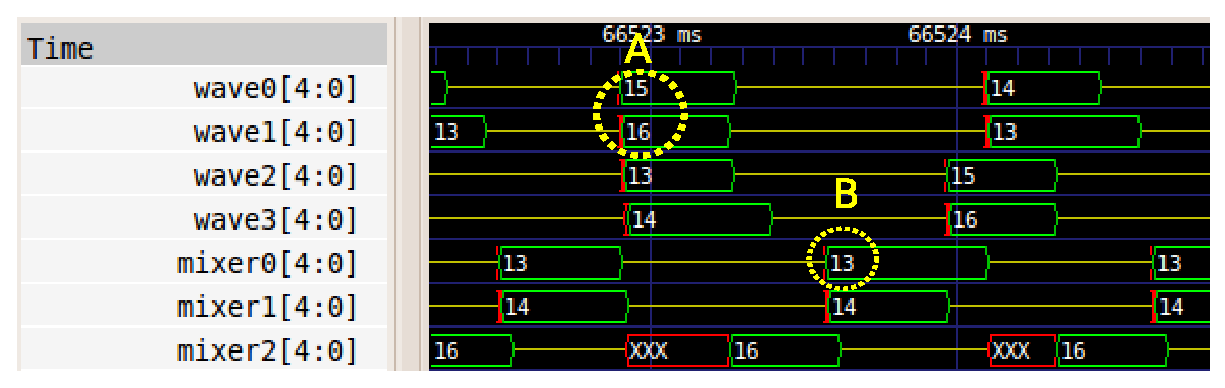
\includegraphics[width=\widefigure]{images/results_AMD/final_AMD.eps}
\caption{\figurecaption{Scheduling performed by new version of task-affinity on Opteron (new version of task-affinity)}}
\label{fig:trace_AMD}
\end{figure}

\begin{figure}[htbp]
\centering
\includegraphics[width=\widefigure]{images/results_AMD/time_avg_var_AMD.eps}
\caption{\figurecaption{Average and Variance of execution time of a sample Opteron (new version of task-affinity)}}
\label{fig:time_avg_var_AMD}
\end{figure}

Task-affinity on this machine doesn't work properly. We can see in step B that \textit{mixer0} doesn't choose the correct CPU. The incorrect behaviour of 
task-affinity is also reflected by Fig. \ref{fig:time_avg_var_AMD}, where we can see a worsening of throughput and predictability. It is possible that the 
task-affinity doesn't work, because of a lot of kernel threads used to manage load balancing and others kernel activities in NUMA architectures: but this is 
only an hypothesis. According these results, it is clear that task-affinity needs the support for NUMA architectures, this is the first step to improve 
task-affinity.

In this work, we have seen that cache misses have a different impact on determinism of application on different architectures, it is necessary to 
estimate how much cache misses impact on application performance and in particular on determinism, in order to understand if the task-affinity could 
improve significantly or not the determinism of application on a given architecture. 

Another possible improvement is to optimize the migration policy, in order to include also \textit{pull\_rt\_task} in task-affinity logic and finally, it 
would be better not to use system calls to define dependencies among tasks, but, instead, to rely in other mechanisms, such as a profiler \cite{calandro}, 
that infers automatically the dependencies among tasks. The reason is that it is not desirable to modify present applications to use the task-affinity. 
The mechanism of adding and removing dependencies would be rather the same: only the user interface would need to be changed.


\newpage

\cleardoublepage
\chapter{Estratto in lingua italiana}
\label{cha:Rev_Italian}

TODO 

\section{Stato dell'arte}
\label{sec:StateDellArte}

\section{Obiettivi di questa tesi}
\label{sec:ObbiettiviTesi}

\section{Organizzazione della tesi}
\label{sec:OrganizzazioneTesi}



%TODO 

\section{Stato dell'arte}
\label{sec:StateDellArte}

\section{Obiettivi di questa tesi}
\label{sec:ObbiettiviTesi}

\section{Organizzazione della tesi}
\label{sec:OrganizzazioneTesi}





% \clearpage 
% \newpage
\cleardoublepage

%\begin{appendices}
%
%\include{a1/Appendix_LinearProgramming}
%\cleardoublepage
%\end{appendices}
%\cleardoublepage
%\chapter{Estratto in lingua italiana}
\label{cha:Rev_Italian}

TODO 

\section{Stato dell'arte}
\label{sec:StateDellArte}

\section{Obiettivi di questa tesi}
\label{sec:ObbiettiviTesi}

\section{Organizzazione della tesi}
\label{sec:OrganizzazioneTesi}



%TODO 

\section{Stato dell'arte}
\label{sec:StateDellArte}

\section{Obiettivi di questa tesi}
\label{sec:ObbiettiviTesi}

\section{Organizzazione della tesi}
\label{sec:OrganizzazioneTesi}





% \clearpage 
% \newpage
%\cleardoublepage


\begin{btSect}[phjcp]{thesis}
 \chapter*{Bibliography}
 \btPrintAll
\end{btSect}

\begin{btSect}[phjcp]{weblinks}
 \chapter*{Webography}
 \btPrintAll
\end{btSect}


\end{document}

